\documentclass[12pt]{article}
\usepackage[letterpaper, top=1.25in, bottom=1.25in, left=1in, right=1in]{geometry}
\usepackage{fancyhdr} % http://ctan.org/pkg/fancyhdr
\usepackage{hyperref}
\usepackage{graphicx}
\usepackage{indentfirst}
\usepackage[export]{adjustbox}
\usepackage{textcomp}
\usepackage{booktabs}

% % % % % % % % % % % % 
% Citation formatting %
% % % % % % % % % % % % 

\usepackage[style=ieee]{biblatex}
\addbibresource{sources.bib}

% % % % % % % % %
% Hyperlinking  %
% % % % % % % % %

\hypersetup{
    colorlinks=false, % set true if you want colored links
    linktoc=all,     % set to all if you want both sections and subsections linked
    % linkcolor=black,  %c hoose some color if you want links to stand out
    % citecolor=black
    % urlcolor=black
}

% % % % % % % % % % % % % % % %
% Global title, author, date  %
% % % % % % % % % % % % % % % %

\title{Conversion Coatings on Non-Ferrous Metals}
\author{Kosta Sergakis}
\date{May 4, 2026}
\makeatletter
\let\runauthor\@author
\let\runtitle\@title
\let\rundate\@date
\makeatother

% % % % % % % % % % %
% Header and Footer %
% % % % % % % % % % %

\pagestyle{fancy} % change page style to fancy
\fancyhf{} % clear header/footer
\setlength{\headheight}{15pt}
\fancyhead[L]{Sergakis}
\fancyhead[C]{\runtitle}
\fancyhead[R]{\rundate}
\fancyfoot[C]{\thepage} % \fancyfoot[R]{\thepage}
\renewcommand{\headrulewidth}{0.4pt} % default \headrulewidth is 0.4pt
\renewcommand{\footrulewidth}{0.4pt} % default \footrulewidth is 0pt

% % % % % % % % % %
% Paper Beginning %
% % % % % % % % % %

% \usepackage{natbib}
\begin{document}
    
    \begin{titlepage}
        \begin{center}
            \vspace*{1.5cm}
            
            \textbf{Exploring Fundamentals of Microstructural Design}
            
            \vspace{1cm}
            
            An exploration of:\\
            \vspace{0.25cm}
            \runtitle
                
            \vspace{1cm}
            
            \textbf{\runauthor}
            
            \vfill  
            
            \vspace{1cm}

            
\includegraphics[width=0.3\textwidth]{resources/michigan-state-logo-png-transparent.png}
                
            Chemical Engineering and Materials Science\\
            Michigan State University\\
            East Lansing, Michigan\\
            \rundate
                
        \end{center}
    
    \end{titlepage}
    
    % % % % % % % % % % %
    % Table of Contents %
    % % % % % % % % % % %

    \setcounter{secnumdepth}{0} % removes section numbers
    % \maketitle
    
    \tableofcontents
    
    \newpage

    \section{Introduction}
        \subsection{Corrosion Issues for Non-ferrous Metals}

            Non-ferrous metals such as aluminum and its alloys, magnesium, zinc, and their coated steels are widely used for transportation, aerospace, construction, and consumer goods because of their high strength-to-weight ratio, formability, and conductivity. Despite forming native oxide films, these metals can suffer significant corrosion in humid, marine, or chemically aggressive environments, leading to loss of mechanical integrity, aesthetic degradation, and premature failure. To meet stringent durability and safety requirements, industries typically rely on multilayer coating systems in which an inorganic conversion layer is a critical pretreatment step beneath paints, sealants, or adhesives \autocite{noauthor_conversion_2018}.

        \subsection{What is a Conversion Coating?}

            In surface treatment, a conversion coating is a thin layer formed on a metal surface by a chemical or electrochemical reaction that converts the outermost metal or its oxide into an adherent, insoluble compound. During this conversion process, metal ions from the substrate and anions from the treatment bath react to produce a new compound layer that is strongly bonded to the base metal, improving corrosion resistance and providing a better key for subsequent organic coatings. Conversion coatings may be generated purely chemically (e.g. chromate or phosphate) or electrochemically (e.g. anodizing) and are essential to achieve robust paint adhesion and long-term protection in demanding applications \autocite{noauthor_conversion_2018}.

            Five major families dominate conversion coating technology for non-ferrous and coated steels: chromate conversion coatings, anodizing of aluminum, zirconium/titanium-based nano-ceramic coatings, silane-based treatments, and phosphate conversion coatings. Each family differs in deposition mechanism, film structure and thickness, typical process steps, and performance trade-offs in terms of corrosion resistance, adhesion promotion, environmental profile, and cost. The following sections examine these systems with emphasis on processing parameters, application areas, and the trends driving a shift toward chromium-free, nano-scale, and hybrid pretreatment stacks.

    \section{Chromate Conversion}
        \subsection{Self-Healing Mechanism}

            \begin{center}
                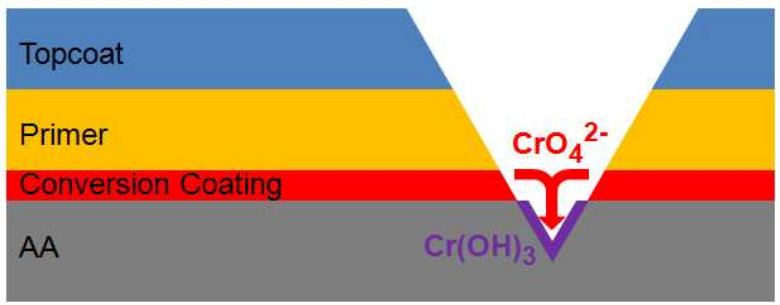
\includegraphics[width=0.75\textwidth]{resources/ccc_diagram.png}
                \\
                \textbf{Figure 1: CCC diagram} \autocite{li_liangliang_corrosion_nodate}
                \label{ccc_diagram}
            \end{center}

            Chromate conversion coatings (CCCs) have historically been the benchmark pretreatment for aluminum and other non-ferrous substrates in aerospace and defense because they combine very good corrosion resistance with a unique self-healing capability. These coatings incorporate hexavalent chromium species, such as chromium and dichromate, which remain partly soluble within the coating and can migrate into damaged areas, where they are reduced and precipitate as protective chromium compounds that repassivate exposed metal \hyperref[ccc_diagram]{[Figure 1]}. As a result, CCCs can inhibit both anodic and cathodic reactions, providing robust protection even when the coating is scratched or partially damaged.

            \hyperref[ccc_diagram]{Figure 1} illustrates a sophisticated multi-layer coating system engineered for \\high-performance aerospace protection, structured to balance physical barrier protection with active chemical repair. At the base of the system lies the conversion coating, which serves as a critical bridge; it replaces the weak native aluminum oxide to ensure the organic primer adheres properly while acting as a chemical reservoir for mobile inhibitor ions \autocite{li_liangliang_corrosion_nodate}. The standout feature of the system depicted in the figure is the "self-healing" mechanism that activates when the coating is physically breached. When a scratch exposes the underlying aluminum, mobile ions stored within the conversion coating (such as chromate, $CrO_4^{2-}$) leach into the local environment and migrate toward the damage. Upon reaching the exposed site, these ions undergo a reduction reaction to form an insoluble, passivating layer (such as chromium hydroxide, $Cr(OH)_3$). This effectively "plugs" the scratch with a new protective film, preventing the corrosion from undermining the rest of the coating.

            \begin{center}
                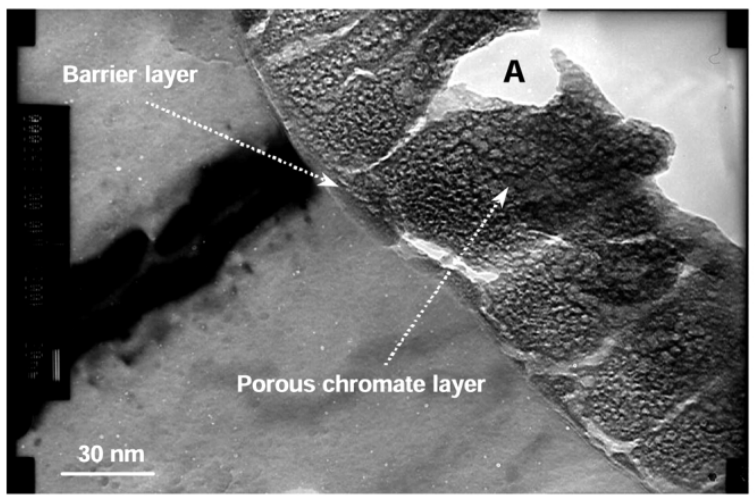
\includegraphics[width=0.5\textwidth]{resources/ccc_cross_section.png}
                \\
                \textbf{Figure 2: TEM micrograph of CCC sample} \autocite{campestrini_study_2002}
                \label{ccc_cross_section}
            \end{center}

            \hyperref[ccc_cross_section]{Figure 2} reveals a distinct, thin, and dense barrier layer situated at the interface between the chromate film and the aluminum substrate. This layer is chemically interpreted as a homogeneous mixture of aluminum and chromium oxide \autocite{campestrini_study_2002}. Beyond this interface, the micrograph shows the bulk chromate film, which contains small pores only a few nanometers in size.

        \subsection{Topographic Development}

            \begin{center}
                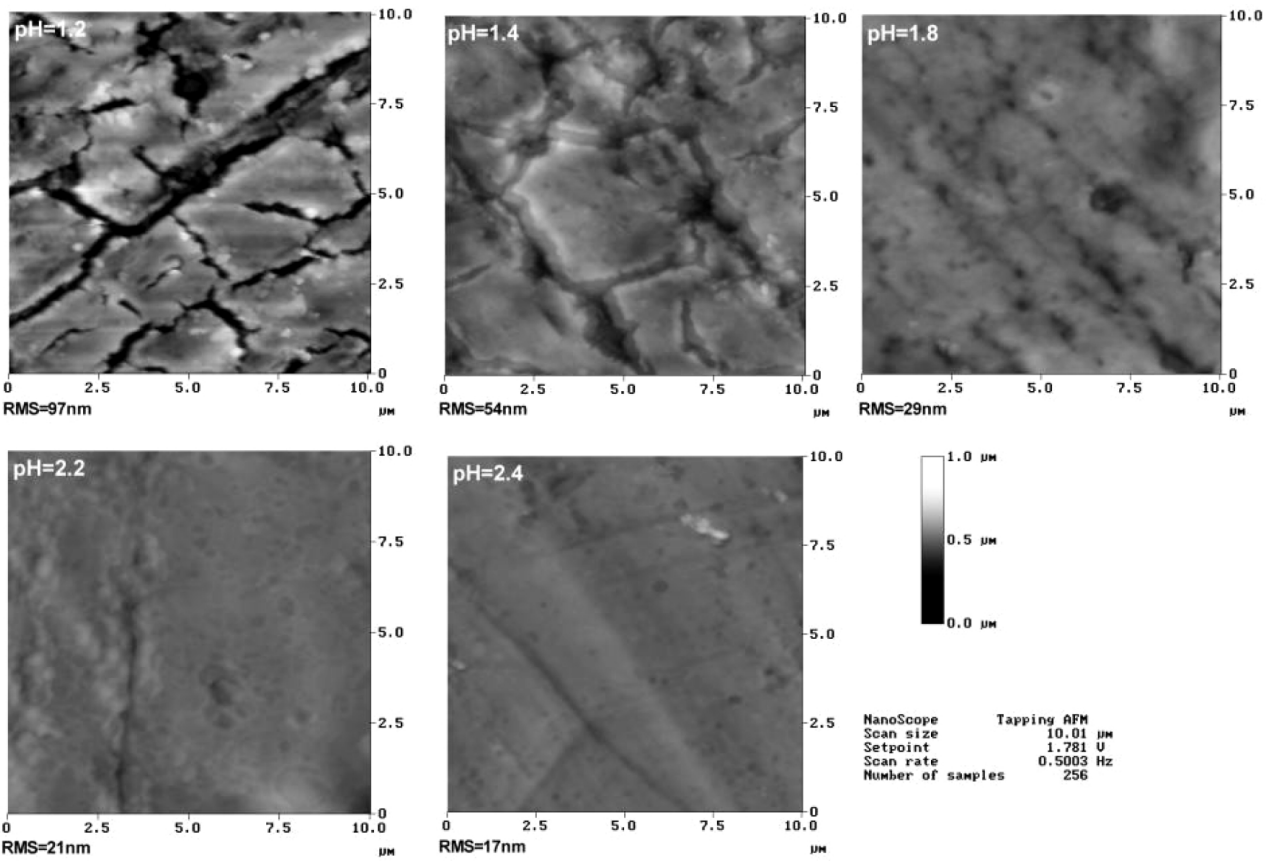
\includegraphics[width=0.9\textwidth]{resources/ccc_afm.png}
                \\
                \textbf{Figure 3: AFM topographic images of chromate conversion coatings obtained at different pH of the chromate bath} \autocite{campestrini_study_2002}
                \label{ccc_afm}
            \end{center}
            
            CCCs are typically applied to cleaned aluminum or other non-ferrous substrates by immersion or spray in acidic chromate-bearing solutions, followed by rinsing and drying. A conventional process sequence consists of alkaline cleaning or degreasing to remove organic soils, a deoxidizing or desmut step if needed, immersion or spray in a chromate conversion bath for a controlled time, water rinsing, and oven or air drying to fix the film. Key parameters include bath pH (often mildly acidic), temperature, time, and chromate concentration, which together determine coating thickness, color, and corrosion performance. Proper control is required to obtain a uniform, adherent film without excessive powdery buildup.

            \hyperref[ccc_afm]{Figure 3} provides a visual and quantitative record of how the acidity of the chromate bath directly dictates the physical texture and density of the resulting protective film. The researchers used these images to calculate the Root Mean Square (RMS) roughness, finding that as the pH of the bath decreases (making it more acidic and aggressive), the surface roughness significantly increases, ranging from a minimum of 27nm at higher pH to a maximum of 97nm at lower pH. This occurs because a more acidic solution etches the aluminum substrate more vigorously, creating a more irregular and porous surface \autocite{campestrini_study_2002}.

        \subsection{Regulatory Evolution}

            The outstanding performance of hexavalent chromate systems is overshadowed by the high toxicity and carcinogenicity of $CR(VI)$ compounds, which has driven strong regulatory pressure under frameworks such as REACH and similar national regulations. Many countries have restricted or phased out traditional $CR(VI)$-based treatments in favor of trivalent chromium systems or completely chromium-free alternatives for most applications, although exemptions persist in some aerospace and defense uses where equivalent performance has been difficult to match. Trivalent chromate conversion coatings and nanoparticle-modified trivalent systems have been developed that can achieve good corrosion resistance and even some degree of self-repair, but they generally require careful process optimization and may not fully replicate the robustness of legacy hexavalent coatings in every environment.

    \section{Anodizing}
        \subsection{Nanoporous Morphologies}

            \begin{center}
                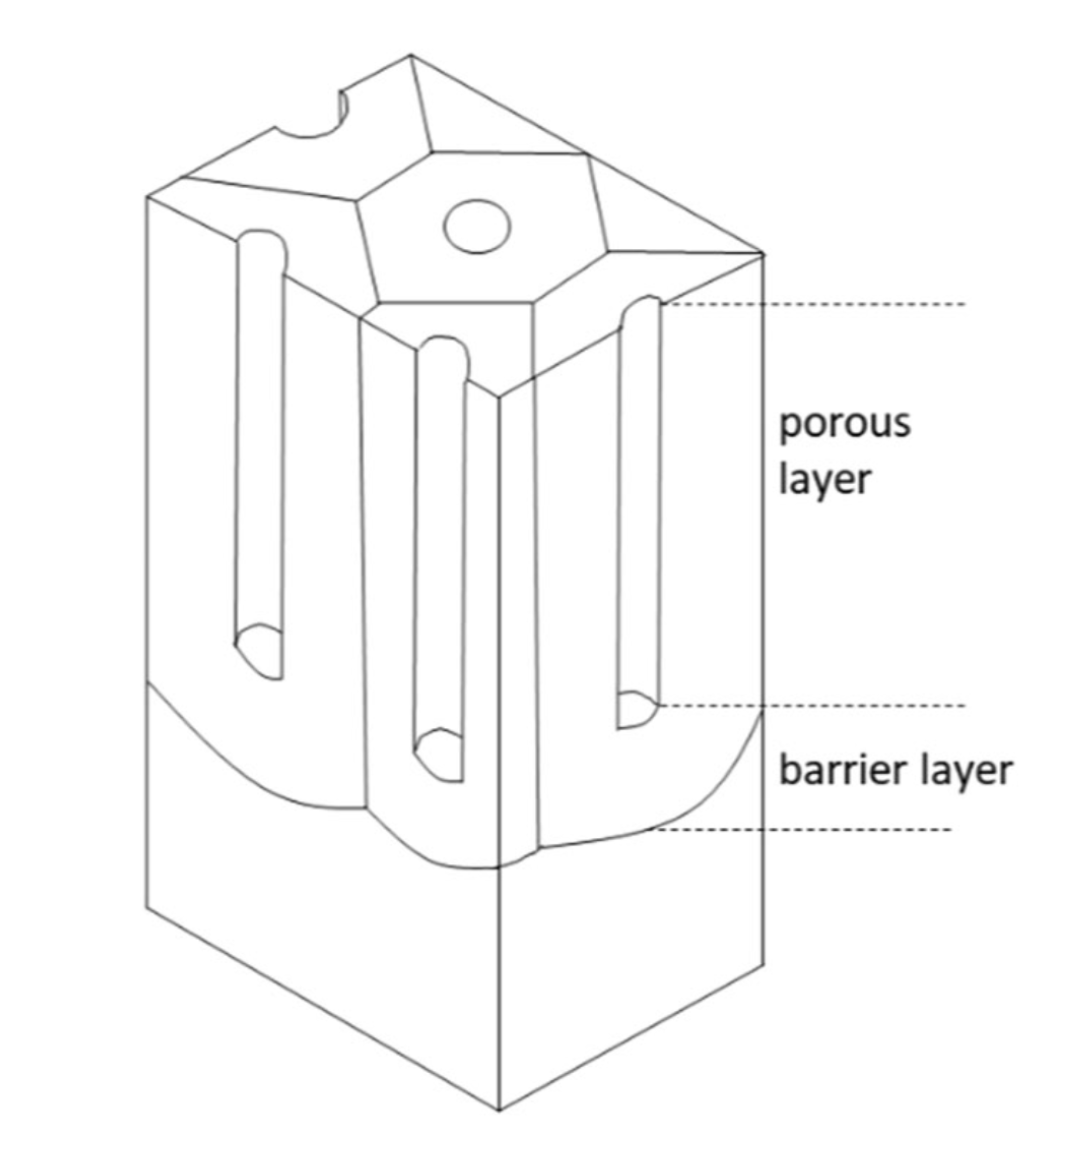
\includegraphics[width=0.35\textwidth]{resources/anodizing_layer_on_aluminum.png}
                \\
                \textbf{Figure 4: Anodizing layer on aluminum} \autocite{schneider_anodizingpore_2022}
                \label{anodizing_layer}
            \end{center}

            Anodizing is an electrochemical conversion process in which the aluminum component is made the anode in an electrolytic cell so that its surface is oxidized to a thick, adherent layer of porous aluminum oxide. Unlike chemical conversion coatings that rely purely on chemical reactions, anodizing uses applied current or voltage to control oxide growth in electrolytes such as sulfuric, chromic, oxalic, or phosphoric acid. The resulting anodic film is typically non-conductive, has well-defined porosity and thickness, and provides an excellent base for coloring and sealing treatments that significantly enhance corrosion and wear resistance.

            \hyperref[anodizing_layer]{Figure 4} illustrates the Keller-Hunter-Robinson (KHR) model, which provides a foundational geometric blueprint for the structure of anodic layers on aluminum. The model depicts coating not as a single uniform slab, but as a dual-structured system consisting of a thin, dense, and pore-free barrier at the metal interface, topped by a significantly thicker porous layer. This porous region is characterized by a series of hexagonal-like "cells," each containing a central, hollow channel known as a nanopore \autocite{schneider_anodizingpore_2022}. According to the text, this model is essential for explaining how the coating continues to grow to micrometer thicknesses; the growth process occurs specifically at the pore bottom, where a delicate balance exists between the electrochemical formation of new oxide and the chemical dissolution (corrosion) caused by the electrolyte.

        \subsection{Layered Growth}

            \begin{center}
                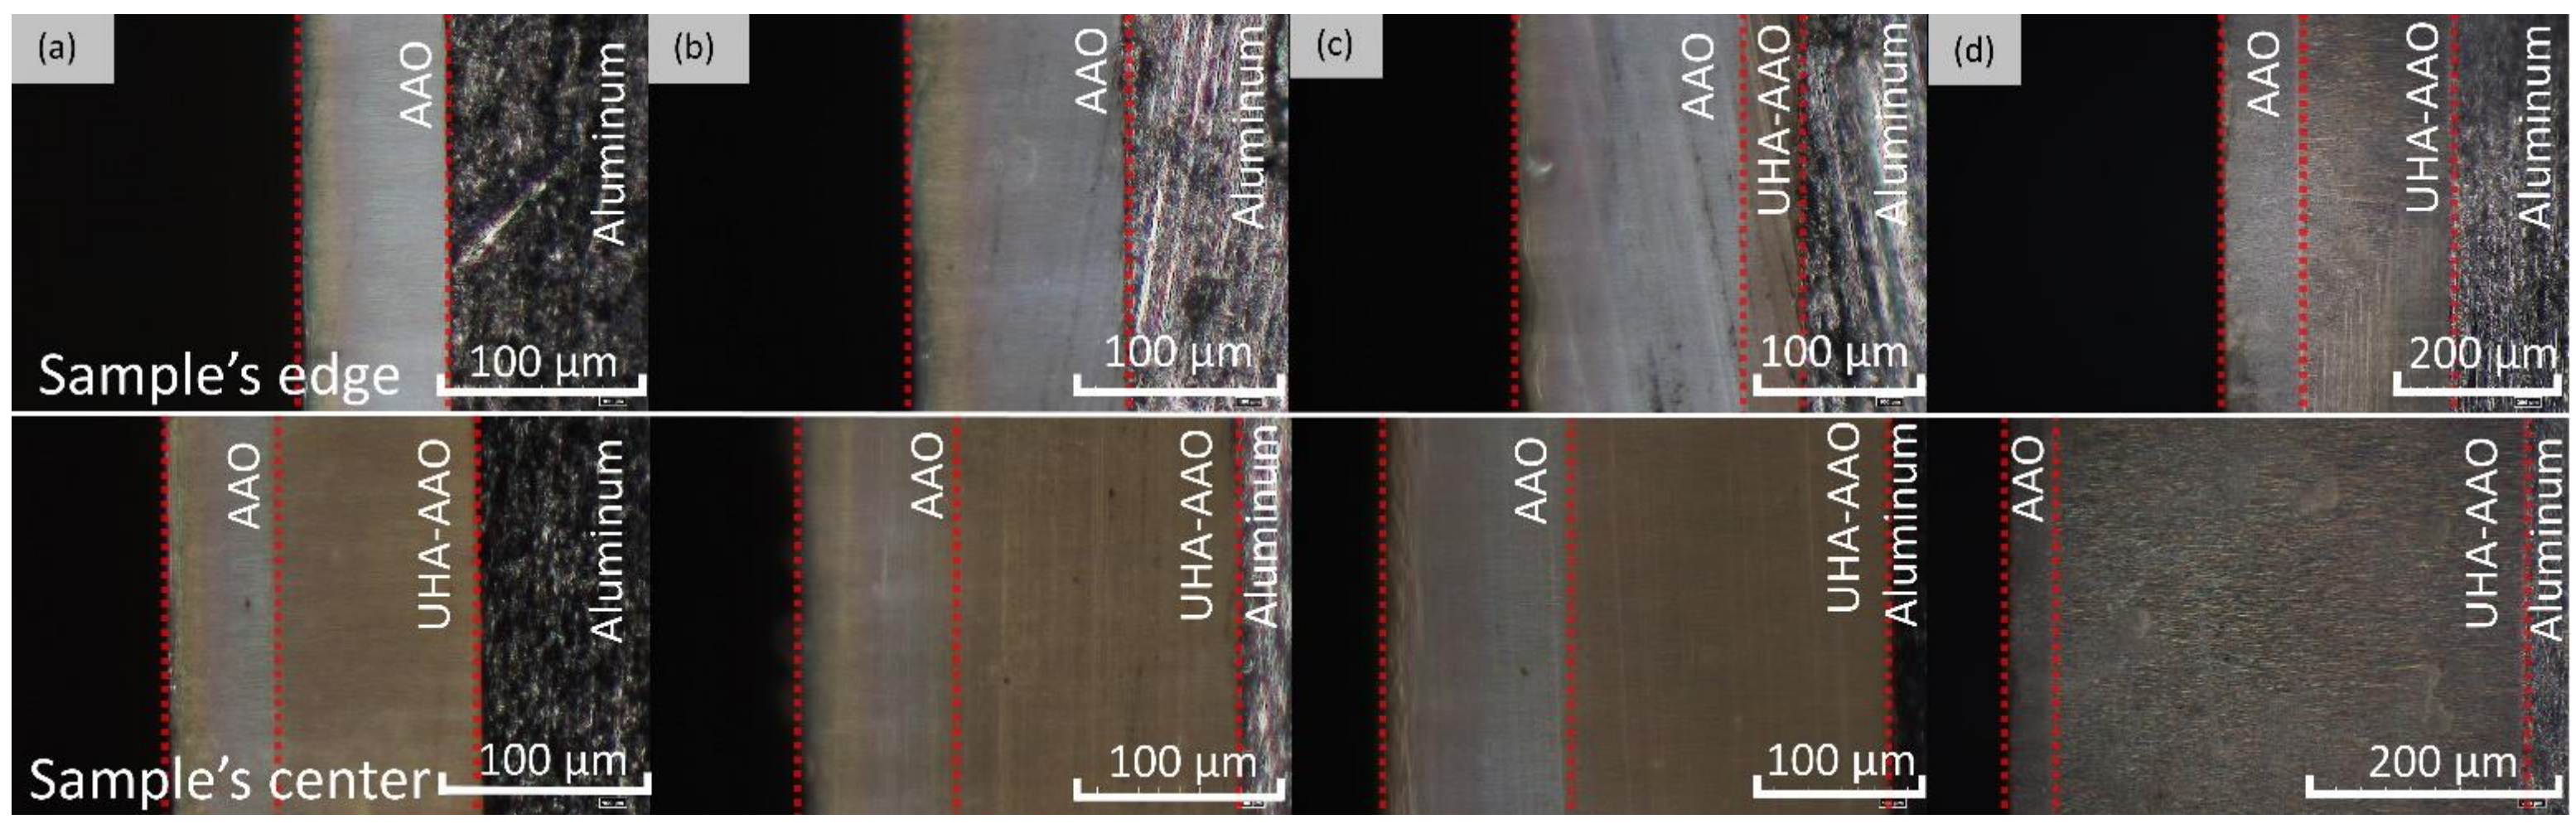
\includegraphics[width=1\textwidth]{resources/anodization_optical_layers_diff_times.png}
                \\
                \textbf{Figure 5: Optical cross-section micrographs of anodized aluminum oxide layer at varying times} \autocite{rozenblium_comprehensive_2024}
                \label{anodizing_layer_dt}
            \end{center}

            A typical anodizing line for aluminum begins with cleaning and degreasing to remove oils, followed by alkaline etching to adjust surface roughness and appearance, and a desmut step to remove intermetallic residues. The parts are then anodized in an acid electrolyte under controlled voltage or current density and temperature, with process recipes varying for sulfuric, chromic, and oxalic acid systems. After anodizing, the porous oxide layer may be dyed or impregnated with pigments for decorative finishes and is usually sealed in hot water or nickel-containing solutions to close the pores and improve corrosion resistance.

            Operating parameters such as acid concentration, bath temperature, current density, and time strongly influence oxide thickness, pore morphology, hardness, and color. Sulfuric acid anodizing (often termed Type II) is the most widely used process for general corrosion protection and decorative coloring, while low-temperature, high-current-density sulfuric processes produce thick "hardcoat" anodic films with high wear resistance (Type III) \autocite{asm_surface_2007}. Chromic acid anodizing has been important in aerospace because of its relatively thin but highly protective films, although environmental concerns over chromic acid have also prompted moves toward sulfuric and mixed-acid alternatives.

            \hyperref[anodizing_layer_dt]{Figure 5} provides a chronological visual record of the Anodized Aluminum Oxide (AAO) coating's internal development through optical cross-section micrographs taken at one, two, four, and six-hour intervals. These images reveal a complex, multi-layered architecture consisting of an initial pre-anodization layer, a standard gray AAO layer, and a distinct brown layer attributed to Ultra-Hard Anodization (UHA). The micrographs demonstrate that the UHA-AAO layer grows at a significantly higher rate than the common AAO layer and gradually expands from the center of the sample toward the edges over time. This layered and non-uniform growth serves as evidence of the thermal imbalances within the reaction zone; specifically, localized heating in the sample's center facilitates the transition to the more intensive UHA growth, while the edges remain cooler and exhibit standard growth \autocite{rozenblium_comprehensive_2024}.

        \subsection{Functional Surface Engineering}

            Anodizing is extensively used for decorative and architectural aluminum, where colored and sealed oxide layers provide both appearance and durability for fa\c{c}ade elements, consumer products, and electronics housings. Hard anodizing is applied to components requiring high abrasion resistance, such as hydraulic cylinders, piston surfaces, and machine parts. In aerospace, anodizing often competes with chromate conversion coatings, with chromic or sulfuric anodizing used on structural aluminum parts as a base for primers and paints, while CCCs are favored where electrical conductivity or minimal dimensional change is needed. In many cases, anodizing and conversion coatings are complementary options within the same platform, selected based on geometry, required conductivity, fatigue performance, and coating system design \autocite{asm_surface_2007}.

    \section{Zirconium/Titanium "Nano-ceramic" Conversion}
        \subsection{Nanometer-Scale Inorganic Architecture}

            \begin{center}
                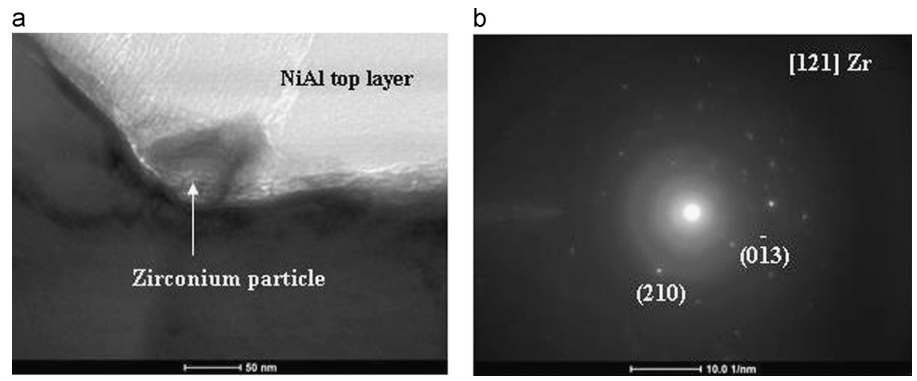
\includegraphics[width=1\textwidth]{resources/nanoparticle.png}
                \\
                \textbf{Figure 6: TEM image of zirconium enriched particles (a) and diffraction pattern of the zirconium enriched particle (b)} \autocite{zagula-yavorska_nanoparticles_2015}
                \label{nano}
            \end{center}

            Zirconium and Titanium-based "nano-ceramic" conversion coatings have gained prominence over the last two decades as chromium-free alternatives to traditional zinc phosphates and Cr(VI) chromates, particularly in automotive body shops and appliance manufacturing. These systems form extremely thin, inorganic films on steel, galvanized steel, and aluminum that are designed to deliver comparable paint adhesion and corrosion resistance while significantly reducing environmental burden and sludge generation. Automotive OEMs have increasingly adopted Zr/Ti-based pretreatments to lower energy consumption, water usage, and waste-treatment costs, while still meeting stringent corrosion warranties for multi-metal bodies.

            The structural findings regarding zirconium nanoparticles in aluminide coatings provide a critical scientific basis for the performance of modern Zr/Ti-based "nano-ceramic" conversion coatings used in automotive and appliance manufacturing. Just as \hyperref[nano]{Figure 6} confirms that zirconium can form stable, nano-scale hexagonal structures that improve oxide adhesion and inhibit sub-scale cavities, these commercial pretreatments leverage similar "nano-ceramic" mechanisms to create a robust chemical bridge between metal substrates and organic paints. By replacing bulkier, environmentally hazardous chromates with these precisely engineered Zr/Ti films, manufacturers achieve a dense, inorganic barrier that mimics the self-passivating qualities found in Zr-doped superalloys \autocite{zagula-yavorska_nanoparticles_2015}.

        \subsection{Hydrolytic Deposition}

             \begin{center}
                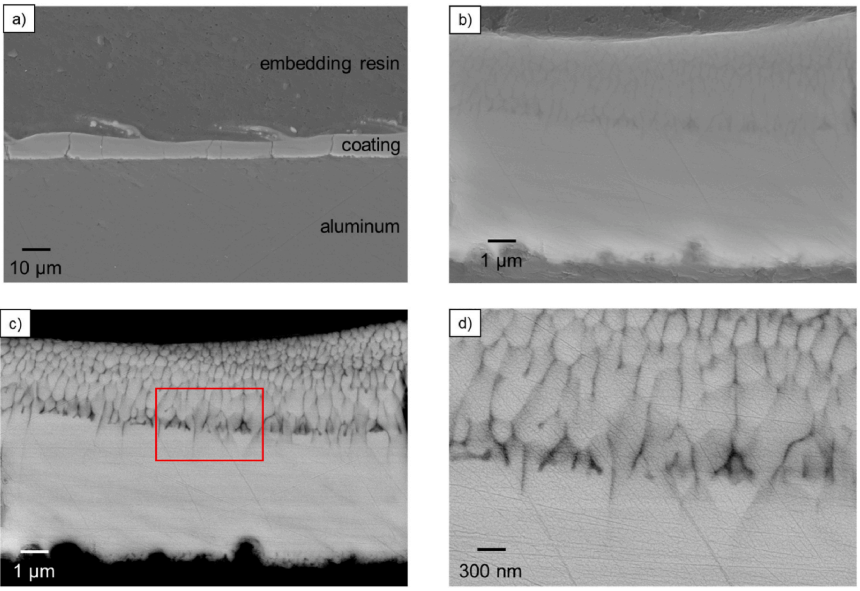
\includegraphics[width=0.8\textwidth]{resources/ceramic_coating.png}
                \\
                \textbf{Figure 7: a) and b) cross-section SEM micrographs of the $Al$/$ZrO_{2}$-filled organosilazane composite coating after laser pyrolysis with different magnifications; c) morphology and solidification structure of laser pyrolyzed $Al$/$ZrO_{2}$-filled organosilazane composite coating; d) enlarged section (red rectangle in c)) of the transition from planar to dendritic solidification structure} \autocite{horcher_advanced_2022}
                \label{ceramic}
            \end{center}

            Zr/Ti nano-ceramic coatings are typically applied from acidic, often fluoride-containing solutions onto thoroughly cleaned metal surfaces by spray or immersion. During treatment, hydrolysis and condensation reactions lead to deposition of nanometer-scale oxide or oxyfluoride species of zirconium and/or titanium that bond strongly to the metal surface and its native oxide. Process control focuses on maintaining the correct pH range, metal ion concentration, and free fluoride, as well as controlling immersion time and bath temperature, because small deviations can markedly alter coating weight and morphology. These baths generally operate at lower temperatures and yield much lower coating weights than conventional phosphates, resulting in less sludge formation, reduced chemical consumption, and easier maintenance.

            \hyperref[ceramic]{Figure 7} provides a STEM-HAADF (High-Angle Annular Dark-Field) image accompanied by chemical maps that visualize the elemental distribution across the cross-section of the zirconium-doped coating. This imaging technique is particularly effective because it uses "Z-contrast," where brighter areas indicate the presence of heavier elements \autocite{horcher_advanced_2022}. The figure confirms the presence of distinct phases, specifically the $\beta$-$NiAl$ and $\gamma$\'-$Ni_{3}Al$ layers, and highlights the shift in aluminum and nickel concentrations between them. Crucially, the oxygen map in \hyperref[ceramic]{Figure 7} reveals the presence of oxygen within Kirkendall-like voids at the interfaces, indicating where internal oxidation or trapped species may reside. While the zirconium signal in this specific bulk preview appears weak, the maps successfully prove that the co-deposition process distributed the reactive elements throughout the depth of the coating \autocite{horcher_advanced_2022}. 
            
            The sensitivity of the coating morphology to chemical conditions shown in \hyperref[ceramic]{Figure 7} parallels the operational requirements of modern Zr/Ti nano-ceramic conversion coatings. Just as the research paper emphasizes that the formation of the $\beta$-$NiAl$ and $\gamma$\'-$Ni_{3}Al$ phases depends on precise temperature and diffusion rates, commercial Zr/Ti systems rely on the delicate balance of hydrolysis and condensation reactions within the acidic, fluoride-containing baths. In both cases, the presence of fluoride is essential: not only for etching the native oxide to "activate" the surface, as seen in the research's deposition stages, but also for controlling the precipitation of nanometer-scale oxyfluoride species \autocite{horcher_advanced_2022}. The "Kirkendall-like" porosity and interface flatnesses observed in the micrographs highlight why industrial process control must be so stringent; small deviations in pH or ion concentration can alter the coating weight and the "nano-ceramic" morphology, potentially leading to the types of voids or non-uniformities that these systems are specifically designed to minimize.

        \subsection{Environmental Performance}

            The films produced by Zr/Ti conversion baths are extremely thin. They are often only a few tens of nanometers, yet they provide excellent paint adhesion and good overall corrosion performance when used as part of a modern paint stack. Their nano-structured, inorganic nature enables intimate contact with both substrate and primer, and the absence of heavy metals and phosphates improves the environmental footprint of the pretreatment line. Laboratory and field data show that Zr/Ti nano-ceramic coatings can match or even surpass zinc phosphate performance for many automotive applications, provided that upstream cleaning and process parameters are tightly controlled.
    
    \section{Silane-based Coatings}
        \subsection{Interfacial Architecture}

            \begin{center}
                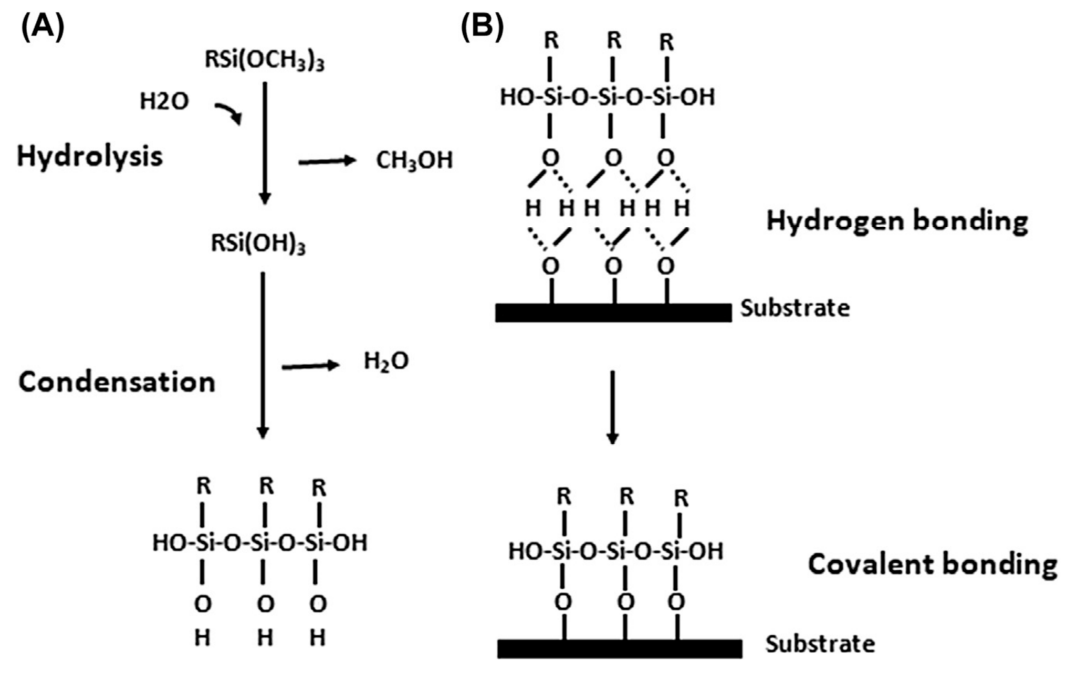
\includegraphics[width=0.8\textwidth]{resources/silane_string.png}
                \\
                \textbf{Figure 8: Hydrolysis and condensation of alkoxysilane and bonding of silanol to the metal substrate. (A) Hydrolysis and condensation to form oligomers in the silane solution and (B) adsorption to an inorganic substrate (such as ceramics or surface or surface oxide layers on metals) by hydrogen bonding and then covalent bonding to the substrate by a condensation reaction with hydroxyl groups} \autocite{al-saadi_silane_2022}
                \label{silane_string}
            \end{center}

            Silane-based coatings use organofunctional silane molecules as coupling agents that can covalently bond to metal oxides and organic matrices simultaneously. After hydrolysis, trialkoxysilanes form silanol groups that react with hydroxylated metal surfaces to create Si-O-metal bonds, while their organic functional groups, such as epoxy, amino, or vinyl, co-react with resins in paints or adhesives \hyperref[silane_string]{[Figure 8]}. This dual reactivity enables silane films to act as both adhesion promoters and, when properly formulated, corrosion-inhibiting pretreatments that can partially or fully replace chromates in some systems.
            
            \begin{center}
                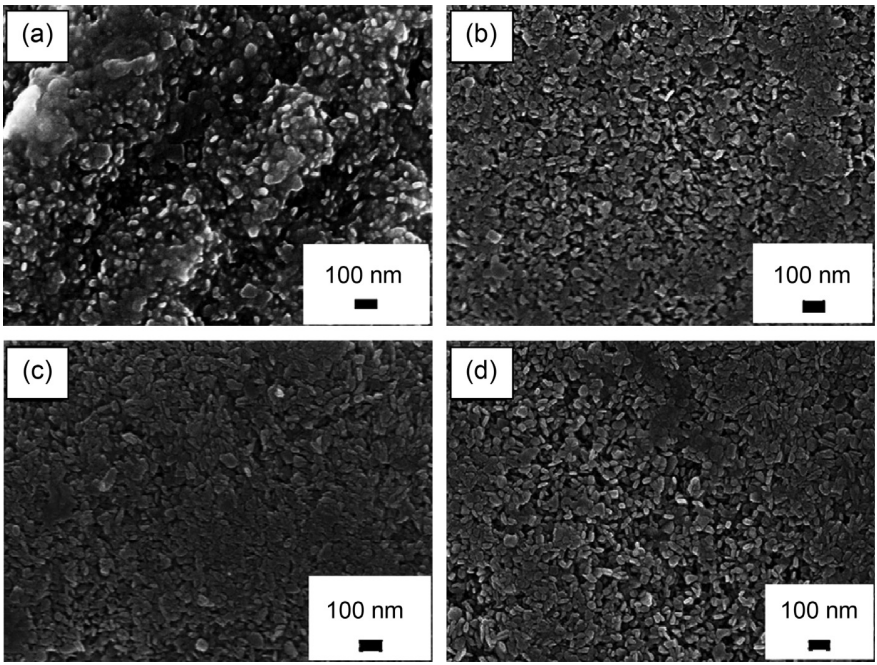
\includegraphics[width=0.72\textwidth]{resources/silane.png}
                \\
                \textbf{Figure 9: Surface morphology of the magnnesium hydroxide coating depositied on an AZ31 magnesium alloy after hydrothermal treatment using 5.66wt\% sodium hydroxide at 160\textdegree C for 1h (a), 2h (b), 3h (c), and 4h (d)} \autocite{narayanan_surface_2015}
                \label{silane}
            \end{center}

            The integration of silane-based treatments depends heavily on the presence of a hydroxylated metal surface to initiate the formation of covalent bonds. As shown in \hyperref[silane]{Figure 9}, the surface morphology of a magnesium alloy can be intentionally modified via hydrothermal treatment to create such a foundation. The figure demonstrates the growth of a magnesium hydroxide ($Mg(OH)_{2}$) coating that becomes increasingly dense and structured as treatment time progresses from one to four hours. By providing a uniform and compact layer rich in hydroxyl groups, this hydrothermal modification creates an ideal substrate for the silanol groups mentioned previously to reach and anchor. This synergy allows the silane coupling agents to bridge the gap between the structured hydroxide layer and an organic matrix, effectively utilizing the physical coverage shown in \hyperref[silane]{Figure 9} to enhance the overall mechanical and chemical stability of the bond.

        \subsection{Hydrolysis-Condensation}

            \begin{center}
                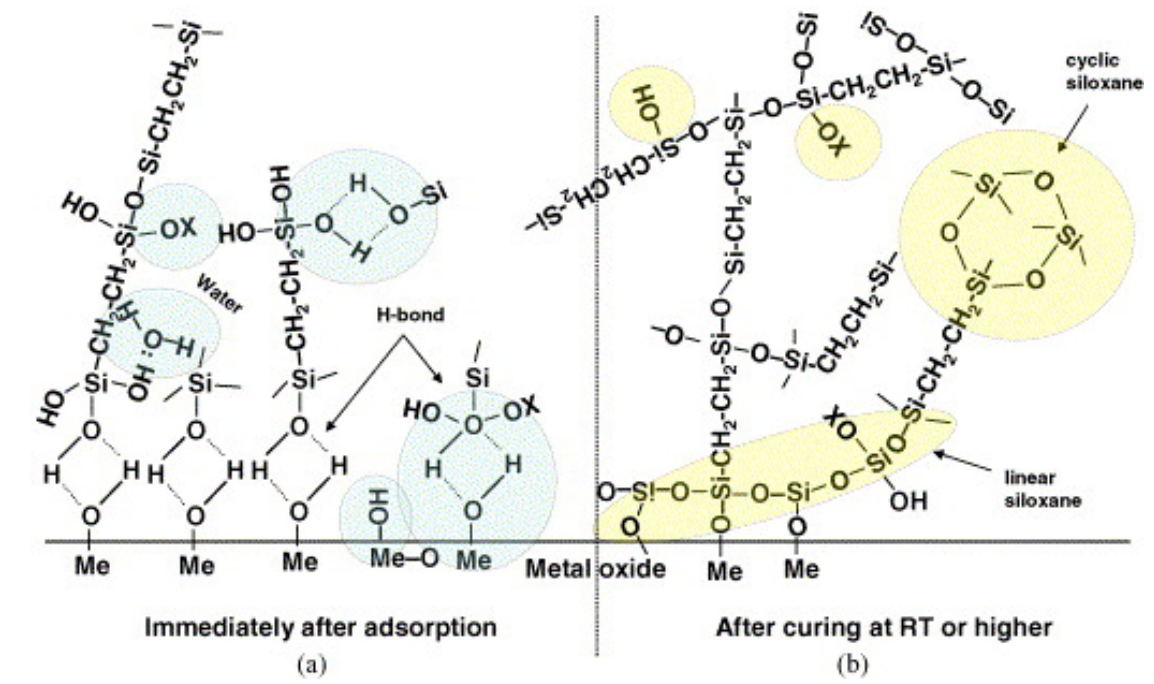
\includegraphics[width=0.8\textwidth]{resources/silane_process.png}
                \\
                \textbf{Figure 10: Simplified schematic of bonding mechanism between silane molecules and metal surface hydroxide layer: (a) before condensation: hydrogen-bonded interface; (b) after condensation: covalent-bonded interface} \autocite{al-saadi_silane_2022}
                \label{silane_process}
            \end{center}

            Silane pretreatments are generally applied from aqueous-alcohol solutions containing one or more silane precursors, often at acidic pH, onto clean and mildly activated metal surfaces. Application may be dipping, spraying, or roll-coating, followed by draining, ambient drying, and thermal curing to drive condensation reactions and form a crosslinked, nanometer-thick siloxane network. Key variables (such as silane concentration, solution pH, hydrolysis time, and curing temperature) affect film uniformity, porosity, and crosslink density, which in turn determine barrier properties and the strength of adhesive bonding.

            The effectiveness of these nanometer-thick siloxane networks is fundamentally rooted in the transition from physical adsorption to chemical integration, a process visually represented in \hyperref[silane_process]{Figure 10}. As illustrated in the schematic, the initial contact between the hydrolyzed silane molecules and the metal surface hydroxide layer is characterized by a hydrogen-bonded interface \hyperref[silane_process]{[Figure 10a]}, where the molecules align but have not yet achieved a permanent structure. It is through the subsequent drying and thermal curing process (often referred to as condensation) that this interface is transformed. As shown in \hyperref[silane_process]{Figure 10b}, the loss of water during condensation converts those temporary hydrogen bonds into a robust, covalent-bonded interface defined by metallo-siloxane (Me-O-Si) bonds. This transition is what allows the film to evolve from a simple wet layer into a crosslinked, hydrophobic barrier that is capable of providing both high-strength adhesive bonding and long-term corrosion protection.

        \subsection{Hybrid Systems and Multi-Material Adhesion}

            Silane-based coatings are used as standalone pretreatments or as components of hybrid systems that combine inorganic nano-ceramic or phosphate layers with an organic silane network to maximize adhesion and corrosion resistance. On aluminum automotive body sheets and aerospace alloys, silane sol-gel films have been shown to improve barrier properties and filiform corrosion resistance under cataphoretic paints and to enhance adhesion in metal-adhesive-composite joints. On steels, eco-friendly silane formulations have demonstrated very high corrosion inhibition efficiency in aggressive chloride environments, making them attractive low-toxicity alternatives to chromate and phosphate for infrastructure and marine applications when paired with suitable topcoats.

    \section{Phosphate Conversion Coatings}
        \subsection{Polycrystalline Morphology}

            \begin{center}
                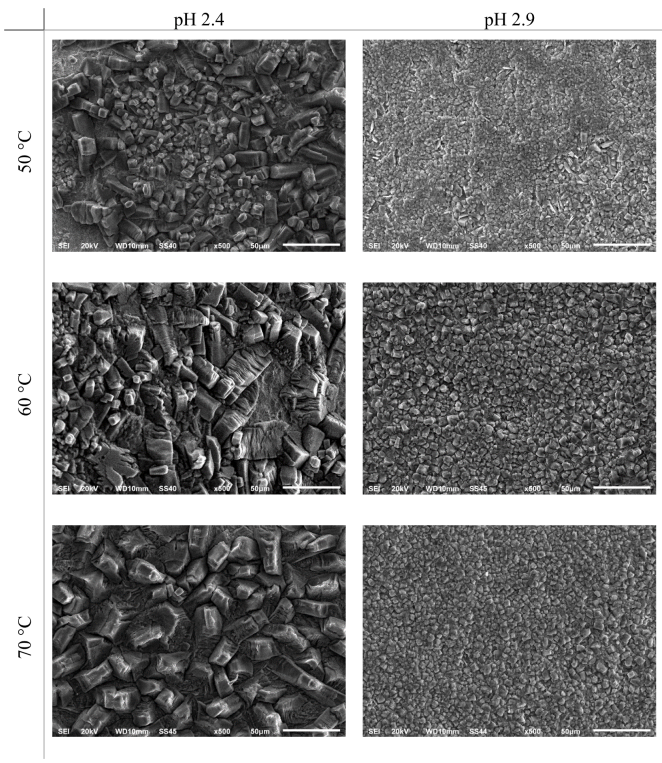
\includegraphics[width=0.65\textwidth]{resources/phosphate.png}
                \\
                \textbf{Figure 11: SEM images of the phosphate films obtained at the indicated temperature and pH} \autocite{silva-fernandez_influence_2023}
                \label{phosphate}
            \end{center}

            Phosphate conversion coatings are among the most widely used pretreatments for steel and are also applied, with adaptations, to galvanized and aluminum substrates in automotive, appliance, and general industrial painting operations. In these processes, the metal surface is chemically converted into a polycrystalline layer of metal phosphates (typically zinc, iron, or manganese) that improves corrosion resistance, provides a strong base for paints, and, in the case of manganese phosphate, can enhance lubricity for cold forming. Zinc phosphate coatings are especially important as paint bases because their microcrystalline structure and incorporation of cations such as zinc, manganese, nickel, and sometimes cobalt give good alkaline resistance and excellent paint adhesion.

            The effectiveness of these polysrystalline layers as a paint base is highly dependent on the resulting morphology and crystal refinement of the film. As demonstrated in \hyperref[phosphate]{Figure 11}, the physical structure of the phosphate coating is sensitive to both the bath temperature and the pH level during the conversion process. At a lower pH of 2.4, the SEM images reveal a mixture of large prismatic and smaller cubic crystals, which can lead to incomplete surface coverage or "uncoated areas" at lower temperatures. However, when the bath is alkalinized to pH 2.9, \hyperref[phosphate]{Figure 11} shows a significant refinement in crystal size (approximately 5$\mu$m), resulting in a more uniform, microcrystalline structure. This compact morphology is essential for the automotive and appliance industries mentioned previously, as it ensures that the metal surface is fully shielded and optimized for subsequent paint adhesion.

        \subsection{Multi-Stage Deposition}

            \begin{center}
                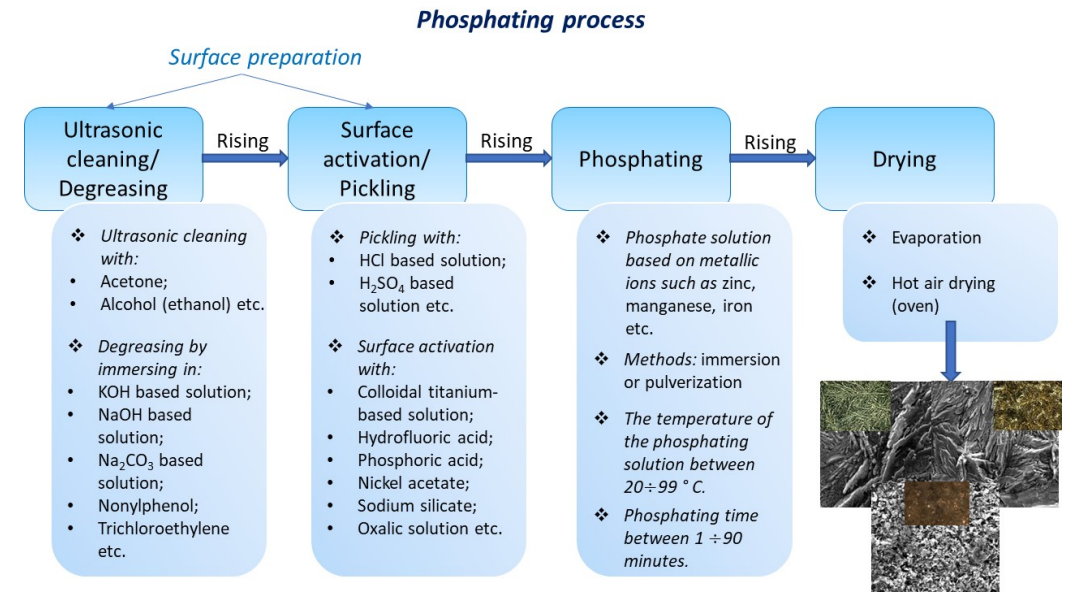
\includegraphics[width=1\textwidth]{resources/phosphate_process.png}
                \\
                \textbf{Figure 12: The phosphating process} \autocite{vizureanu_phosphate_2023}
                \label{phosphate_process}
            \end{center}

            Phosphate coatings are formed by applying dilute phosphoric-acid-based solutions containing appropriate metal ions to the substrate by spray or immersion. A typical sequence consists of cleaning and degreasing, activation or grain refinement (for many zinc phosphate processes), phosphating under controlled temperature and acidity, rinsing, and sometimes post-treatment with sealers. Bath chemistry and operating parameters (temperature, total and free acidity, accelerator content, and treatment time) govern coating weight, crystal size, and uniformity, which directly influence corrosion performance and paint adhesion. Modern automotive lines often employ tri-cationic phosphate baths that deposit polycrystalline coatings containing zinc, nickel, and manganese on steel, galvanized steel, and aluminum, enabling multi-metal pretreatment in a single process.

            The close control of these chemical parameters and process variables is essential for transitioning from a raw metal substrate to a protected, high-performance surface. This systematic progression is visually summarized in \hyperref[phosphate_process]{Figure 12}, which outlines the integrated stages of the phosphating process along with the specific chemical agents and characterization techniques involved. As illustrated in the diagram, the journey begins with surface preparation (using ultrasonics, alkaline degreasers like $KOH$, or acid pickling) to ensure the substrate is chemically active and free of contaminants. Following activation with agents such as colloidal titanium, the material enters the phosphating stage, where immersion or spraying at temperatures typically between 30\textdegree C and 60\textdegree C initiates the formation of the conversion layer. \hyperref[phosphate_process]{Figure 12} further contextualizes these results by showcasing SEM and Optical Microscopy images, highlighting how variations in bath composition and additives directly dictate whether the final coating manifests as a coarse crystalline structure for heavy-duty protection or a refined, compact morphology ideal for paint adhesion.

        \subsection{Substrate Versatility}

            Phosphate coatings are the most straightforward on steels, where they naturally form iron or zinc phosphate layers; however, methods have been developed to treat aluminum and galvanized substrates, although coating quality can be more sensitive to alloy composition and surface condition. The phosphating process typically operates at elevated temperatures and produces substantial sludge from precipitation of phosphates and metal salts, increasing maintenance, equipment cleaning, and waste-treatment requirements. As environmental and cost pressures increase, these drawbacks have prompted the search for alternative technologies such as low-temperature, low-sludge Zr/Ti nano-ceramic systems that can deliver similar or better performance with a smaller environmental footprint.

    \section{Comparison, Application, and Trends}

        The conversion coatings discussed - Chromate (CCC), Anodizing, Zirconium/Titanium (Zr/Ti) nano-ceramics, Silanes, and Phosphates - represent a broad spectrum of surface engineering. While they all aim to transform a reactive metal surface into a stable protective layer, they differ significantly in their chemical mechanisms, physical properties, and environmental footprints.

        \subsection{Key Similarities and Differences}

            The primary similarity among these treatments is their interfacial nature: each process chemically or electrochemically alters the substrate rather than simply sitting on top of it. This ensures superior adhesion compared to simple organic coatings.

            However, their mechanisms and structures vary:

            \begin{itemize}
                \item Formation Mechanism: CCC, Zr/Ti, Silanes, and phosphates are chemical immersion or spray processes. In contrast, Anodizing is electrochemical, requiring an external power source to drive the growth of a much thicker and more structured oxide layer.
                
                \item Coating Structure: Phosphates and Anodizing produce relatively thick, porous, and polycrystalline or amorphous structures that are ideal for "anchoring" secondary layers. CCCs and Silanes are much thinner, focusing on chemical passivity. Zr/Ti coatings represent the "nano" extreme, providing high performance with minimal material thickness.
                
                \item Self-Healing: A unique differentiator is the active protection found in Chromate Conversion Coatings. The hexavalent chromium species act as a reservoir that can migrate to repair scratches; a feature largely absent in the purely "passive" barriers formed by Phosphates or Anodizing.
            \end{itemize}
        
        \subsection{Applications by Industry}

            The choice of coating is strictly dictated by the performance requirements of the specific end-use environment:

            \begin{table}[h]
                \centering
                \textbf{Table 1: Conversion coating application by industry}
                \label{coating_applications}
                \resizebox{\textwidth}{!}{%
                    \begin{tabular}{lll}
                        \toprule
                        \textbf{Coating Type} & \textbf{Primary Industry} & \textbf{Key Functional Driver} \\ \midrule
                        Chromate (CCC) & Aerospace \& Defense & Critical corrosion resistance and self-healing. \\
                        Anodizing & Architecture \& Electronics & Aesthetic coloring, wear resistance, and hardness. \\
                        Zr/Ti Nano-ceramic & Automotive (OEM) & Multi-metal lines with zero sludge generation. \\
                        Silanes & Adhesives \& Electronics & Precision bonding of inorganic and organic layers. \\
                        Phosphates & Heavy Industry & Paint pretreatment and cold forming lubricity. \\ \bottomrule
                    \end{tabular}
                }
            \end{table}

            The selection of a conversion coating is a strategic decision governed by the specific environmental and mechanical demands of the end-use application, as detailed in \hyperref[coating_applications]{Table 1}. While heavy industries and appliance manufacturers rely on the microcrystalline structure of phosphates for paint adhesion and cold-forming lubricity, high-performance sectors like aerospace prioritize the active "self-healing" properties of chromates to survive aggressive conditions. Meanwhile, modern automotive manufacturing has shifted toward Zirconium/Titanium "nano-ceramics" to facilitate sustainable, multi-metal processing without the waste-treatment burden of traditional methods. For consumer-facing products, anodizing is the preferred choice for its unique combination of vibrant aesthetics and surface hardness, whereas silane-based systems excel in high-precision electronic or adhesive applications where covalent bonding between dissimilar materials is critical.

        \subsection{Current Trends and Future Outlook}

            The trajectory of conversion coating technology is currently defined by a few major trends:

            \begin{itemize}
                \item Elimination of Hexavalent Chromium: Due to the toxicity and strict regulations surrounding $Cr(VI)$, there is a massive push to replace CCCs. While Zr/Ti and Silanes have successfully replaced chromates in the automotive sector, the aerospace industry is still searching for a chromium-free alternative that matches the "self-healing" reliability of CCC.
                
                \item Sustainability and "Dry-In-Place" Technology: There is a move toward processes that require fewer rinsing stages. Zr/Ti nano-ceramics and Silanes are leading this trend because they generate almost no sludge, reducing the energy and water costs associated with waste treatment in traditional phosphate lines.
                
                \item Multi-Metal Capability: Modern manufacturing often involves assemblies of aluminum, steel, and galvanized steel. Trends favor "universal" pretreatments, like tri-cationic phosphates or Zr/Ti systems, that can react effectively across multiple substrates in a single immersion bath without cross-contaminating the chemistry.
            \end{itemize}
        
            The continuous evolution of conversion coatings represents a critical balance between achieving superior interfacial performance and adhering to increasingly stringent environmental and safety regulations. Ultimately, the industry is transitioning away from legacy heavy-metal chemistries toward nanometer-scale, multi-metal, and "self-healing" alternatives that offer a sustainable pathway for protecting advanced materials without compromising engineering integrity.


    % % % % % % % % %
    % Bibliography  %
    % % % % % % % % %

    % \addcontentsline{toc}{section}{Works Cited}
    % \printbibliography
    \newpage
    \phantomsection % Create a phantom section to get the correct page number in the ToC
    \addcontentsline{toc}{section}{Works Cited}
    \printbibliography[title=Works Cited]

    % \bibliographystyle{plainnat}
    % \bibliography{sources}

\end{document}
